\documentclass{beamer}

\DeclareMathOperator*{\argmax}{arg\,max}

\usepackage{graphicx}

\usepackage{slashbox}
\usepackage{arydshln}

\usepackage[noend]{algpseudocode}
\renewcommand{\algorithmicrequire}{\textbf{Input:}}
\renewcommand{\algorithmicensure}{\textbf{Output:}}

\usepackage{listings}
\lstset{basicstyle=\tiny}

\usetheme{Madrid}

\hypersetup{pdfpagemode=FullScreen}

\begin{document}

\title[Parallel Simulation R\&S Procedures]
{
Design and Implementation of Parallel Simulation~Ranking~and~Selection~Procedures
}
\author{WU, Yang}
\institute[IELM, HKUST]
{
  Department of Industrial Engineering and Logistics Management\\
  The Hong Kong University of Science and Technology
}
\date{2, Aug 2013}

\begin{frame}
\titlepage
\end{frame}

\begin{frame}
\frametitle{Outline}
\tableofcontents
\end{frame}

\AtBeginSection[]
{
  \begin{frame}
  \frametitle{Outline}
  \tableofcontents[currentsection]
  \end{frame}
}

\section{Introduction}

\begin{frame}
\frametitle{Original Problem}
\framesubtitle{Problem of Selecting the Best}
\begin{itemize}
\item decide the best one from a finite number of alternatives
\vspace{\baselineskip}
\item the best is defined as the one with the largest or smallest mean, inferred from statistical sampling
\vspace{\baselineskip}
\item sampling by real experiments or computer simulations
\end{itemize}
\end{frame}

\begin{frame}
\frametitle{Original Solution}
\framesubtitle{within Serial Computing Environment}
\begin{itemize}
\item Simulation Ranking-and-Selection(R\&S) Procedures
\begin{itemize}
\item a black-box approach
\item simulate all the alternatives, each for many times
\item collect enough samples and make our decision
\item statistical guarantees of correct selection
\end{itemize}
\vspace{\baselineskip}
\item Serial Simulation R\&S Procedures
\begin{itemize}
\item run simulation, get corresponding sample, do some calculation
\item starts earlier, finish earlier: ``the sequential nature"
\item statistical validity of serial procedure
\end{itemize}
\end{itemize}
\end{frame}

\begin{frame}
\frametitle {Significant Change of Computing Environment}
\framesubtitle{The Age of Parallel Computing}
\begin{itemize}
\item fast-growing of serial execution speed has almost stopped, due to physical limitations
\vspace{\baselineskip}
\item new growing point of computing power relies on multiple parallel execution units
\vspace{\baselineskip}
\item large problem can be divided into smaller ones, and small problems can be executed simultaneously, thus speeding up
\end{itemize}
\end{frame}

\begin{frame}
\frametitle {Significant Change of Computing Environment}
\framesubtitle{Making a impact}
\begin{itemize}
\item Serial Computing Environment
\begin{itemize}
\item program will execute faster as the serial execution speed goes up
\item simulation R\&S procedures will also speed-up naturally, without modifying the design of procedure, even the programming implementation
\end{itemize}
\vspace{\baselineskip}
\item Parallel Computing Environment
\begin{itemize}
\item serial program will {\color{blue} NOT} execute faster with more available parallel execution units, unless get paralleled, explicitly or implicitly
\item serial simulation R\&S procedures, with the ``sequential nature", will {\color{blue} NOT} speed-up either, unless re-designed and re-implemented into parallel
\end{itemize}
\end{itemize}
\end{frame}

\begin{frame}
\frametitle{Extra Consideration of Computing}
\framesubtitle{from Complexity to Scalability}
\begin{itemize}
\item {\bf performance}
\begin{itemize}
\item {\bf response time:} time cost for entire job
\item {\bf throughput:} number of jobs done in one time unit
\end{itemize}
depend on problem size, serial execution speed, number of parallel computing units...
\item {\bf time complexity}
\begin{itemize}
\item an expression in big O notation, representing the total workload against the increasing of problem size
\item independent of serial execution speed
\item without considering number of parallel computing units
\end{itemize}
\item {\bf scalability}
\begin{itemize}
\item the ability of a system utilizing extra parallel computing units
\item also independent of serial execution speed
\item fixed problem size
\end{itemize}
\end{itemize}
\end{frame}

\begin{frame}
\frametitle{Our Work}
\begin{itemize}
\item a parallel framework with good scalability
\vspace{\baselineskip}
\item several simulation experiments and R\&S procedures based on the framework
\vspace{\baselineskip}
\item complexity improvement of a specific R\&S procedure by adopting heap
\end{itemize}
\end{frame}

\section{Existing Procedure Analysis}

\begin{frame}
\frametitle{Staged Procedure}
\framesubtitle{the Rinott's Procedure}
\begin{enumerate}
\item{Set up: } Set up parameters $\alpha$, $\delta$ and $n_0$. $n_0$ is the sample size in first stage and $n_0 \geqslant 2$.
\item{Initialize: } Calculate Rinott's constant $h$ with $n_0, k, \alpha$. Collect $n_0$ independent sample values $X_{ij}$, where $j = 1, 2,...,n_0$, for each alternative $i$, by repeatedly running simulation the alternative, and for $i = 1, 2,...,k$, calculate $S_i^2$. Let 
$ N_i = \max\{n_0, \lceil \frac{h^2S_i^2}{\delta^2} \rceil\} $ where $N_i$ is the number of sample value that will eventually taken from alternative $i$.
\item{Stopping Rule: } If $n_0 \geqslant \max N_i$ then stop and select the alternative with the best sample mean, namely the largest or smallest $\bar{X}_i(n_0)$. Else take $\max\{N_i - n_0, 0\}$ extra sample values from each alternative $i$ by continue repeating the simulation experiments, after which select the alternative with largest or smallest $\bar{X}_i(N_i)$ as the best.
\end{enumerate}
\end{frame}

\begin{frame}
\begin{figure}[ht]
\centering
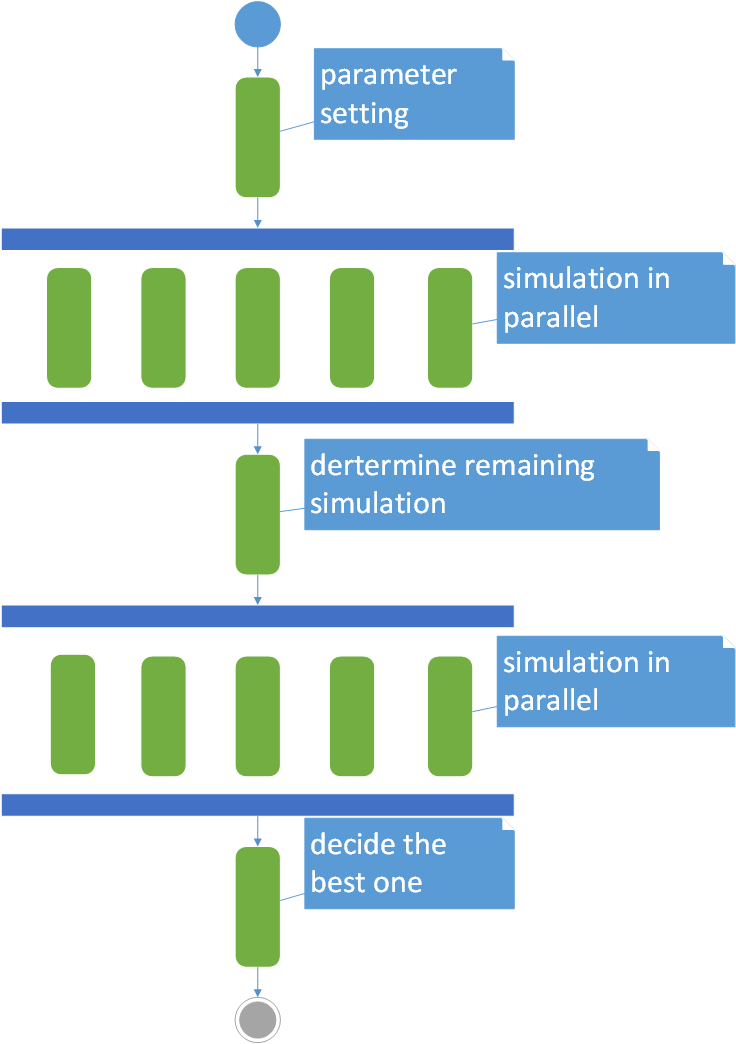
\includegraphics[height=96mm]{rinott_activity.png}
\end{figure}
\end{frame}

\begin{frame}
\frametitle{Redesign of the Rinott's Procedure}
\begin{algorithmic}[1]
\Require $k, \alpha, \delta, n_0$
\State $h \gets$ the Rinott's const with arguments $k, \alpha, n_0$
\State $altIds \gets \{0, 1, 2...k - 1, 0, 1, 2...k - 1...\}$ \Comment{repeat $n_0$ cycles}
\State simulate alternatives with id in $altIds$ \textbf{in parallel}; store result into $X_{ij}$
\State $altIds2 \gets \emptyset$
\For{$i = 0 \to k - 1$}
  \State $\bar{X_i}(n_0) = \frac{1}{n_0} \sum_{j=0}^{n_0 - 1}X_{ij}$;  $S_i^2 = \frac{1}{n_0 - 1} \sum_{j=0}^{n_0 - 1}(X_{ij} - \bar{X_i}(n_0))^2$;
  \State $N_i = \max\{n_0, \lceil \frac{h^2S_i^2}{\delta^2} \rceil\}$
  \For{$j = 0 \to (N_0 - n_0) - 1$}
    \State append $i$ into $altIds2$
  \EndFor
\EndFor
\State simulate alternatives with id in $altIds2$ \textbf{in parallel}; store result into $X_{ij}$
\For{$i = 0 \to k - 1$}
  \State $\bar{X_i}(N_0) = \frac{1}{N_0} \sum_{j=0}^{N_0 - 1}X_{ij}$
\EndFor
\State \Return $\argmax_{i}\bar{X_i}(N_0)$
\end{algorithmic}
\end{frame}

\begin{frame}
\frametitle{Fully Sequential Procedure}
\framesubtitle{the KN Procedure}
\begin{enumerate}
\item{Set up: } Set up parameters $\alpha$, $\delta$, $n_0$ and $h^2 = (n_0 -1)[(\frac{2\alpha}{k - 1})^{-2/(n_0-1)} - 1]$.
\item{Initialize: } Collect $n_0$ independent sample values $X_{i\ell}$, where $\ell = 1, 2,...,n_0$, for each alternative $i$, by repeatedly simulating that alternative, and for $i \neq j$ compute $S_{ij}^2 = \frac{1}{n_0 - 1}\sum_{\ell=1}^{n_0}(X_{i\ell} - X_{j\ell} - [\bar{X_i}(n_0) - \bar{X_j}(n_0)]^2)$, let $r = n_0$.
\item{Elimination: } Set $I^{old} = I$. Let $I = I^{old} - \{i \in I^{old}: \bar{X}_{i\ell}(r) - \bar{X}_{j\ell}(r) < \min\{0, - \frac{h^2S_{ij}^2}{2r\delta} + \frac{\delta}{2} \} \}$
\item{Stopping Rule: } If $|I| = 1$, then stop and select the only surviving alternative, otherwise take another simulation output $X_{i,r+1}$ from each system $i$ and set $r = r + 1$ and go to Elimination.
\end{enumerate}
\end{frame}

\begin{frame}
\begin{figure}[ht]
\centering
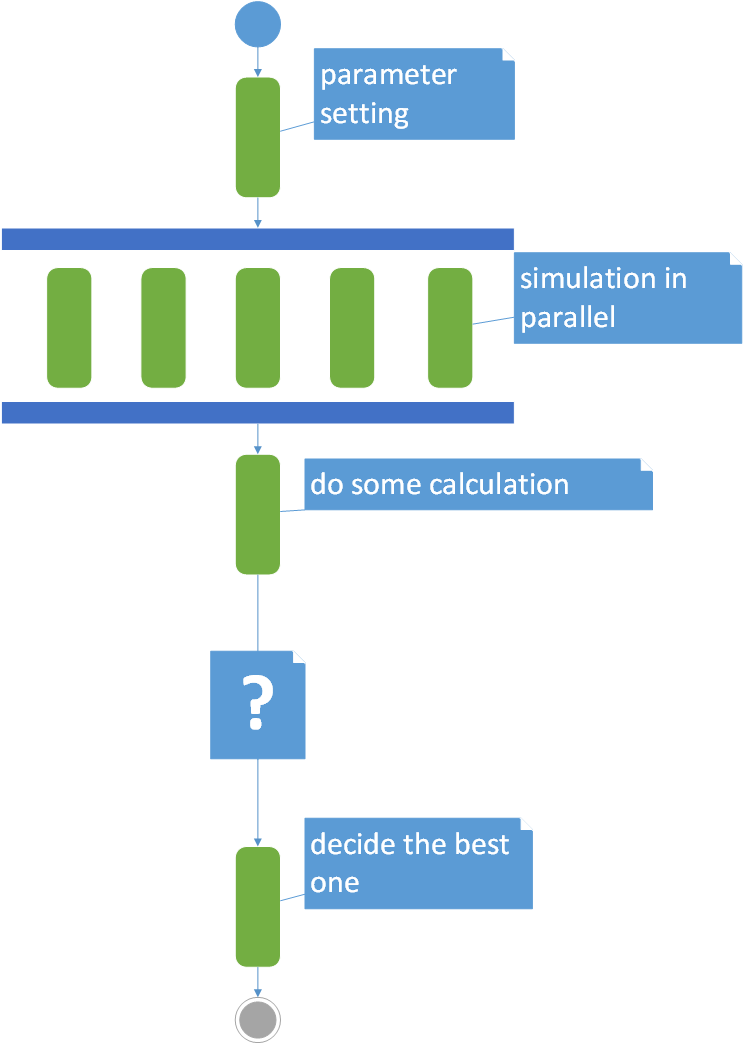
\includegraphics[height=96mm]{kn_activity.png}
\end{figure}
\end{frame}

\begin{frame}
\frametitle{Redesign of Fully Sequential Procedure}
\framesubtitle{Discussion of Sequential Processing}
Why only run simulation one at a time?
\begin{itemize}
\item fork/join again?
\item fork only?
\item Random order of output sequence, violating of the sequential nature.
\end{itemize}
\begin{figure}[ht]
\centering
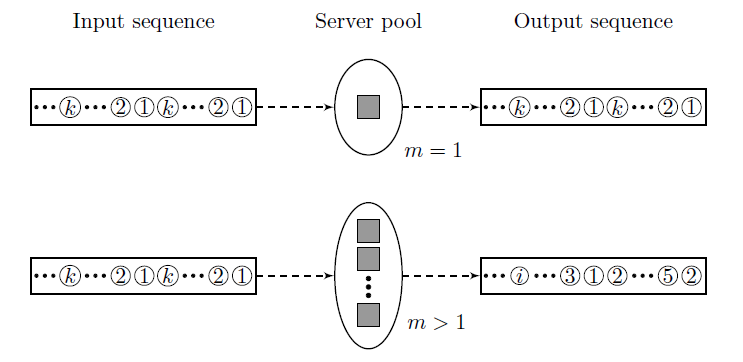
\includegraphics[height=28mm]{queueing.png}
\caption{A Queuing Analogy borrowed from \cite{ras-seq-parallel}:}
\end{figure}
\tiny
{
\begin{thebibliography}{10}
\bibitem{ras-seq-parallel} J. LUO, L. J. HONG, B. L. NELSON, Y. WU. Fully Sequential Procedures for Large-Scale Ranking-and-Selection Problems in Parallel Computing Environments.
\end{thebibliography}
}
\end{frame}

\begin{frame}
\frametitle{Redesign of Fully Sequential Procedure}
\framesubtitle{Discussion of Sequential Processing: cont.}
Why carry out global calculation each time after obtaining a sample value?
\begin{itemize}
\item Global calculation is expensive in parallel computing.
\end{itemize}
\begin{columns}
\column{.05\textwidth}
\column{.45\textwidth}
essential problems:
\begin{itemize}
\item inconsistent read
\item update lost
\end{itemize}
introduced problems:
\begin{itemize}
\item deadlock
\item load imbalance
\item ...
\item performance loss
\end{itemize}
\column{.45\textwidth}
\begin{table}[ht]
\begin{tabular}{|c|c|}
\hline
thread 1 & thread 2 \\
\hline
i++ & i++ \\
\hdashline
read i & \\
calculate i+1 & read i \\
write i+1 to i & calculate i+1 \\
& write i+1 to i \\
\hline
\end{tabular}
\end{table}
\column{.05\textwidth}
\end{columns}
Shall we conduct fewer global calculation?
\begin{itemize}
\item Missing potential elimination chance.
\end{itemize}
\end{frame}

\begin{frame}
\frametitle{Redesign of Fully Sequential Procedure}
\framesubtitle{Vector Filling KN Procedure}
\begin{table}[ht]
\begin{center}
\scalebox{0.8}
{
\begin{tabular}{|c|c|c|c|c|c|}
\hline
\backslashbox{r}{Alternative Id:} & 0 & 1 & 2 & ... & $k - 1$ \\
\hline
1 & $X_{0,1}$ & $X_{1,1}$ & $X_{2,1}$ & ... & $X_{k - 1,1}$ \\
2 & $X_{0,2}$ & $X_{1,2}$ & $X_{2,2}$ & ... & $X_{k - 1,2}$ \\
\hdashline
3 & $X_{0,3}$ & null & $X_{2,3}$ & ... & $X_{k - 1,3}$ \\
4 & $X_{0,4}$ & null & null & ... & null \\
5 & null & null & null & ... & null \\
... & ... & ... & ... & ... & ... \\
\end{tabular}
}
\end{center}
\end{table}
\begin{itemize}
\item track each sample in vector
\item consider the minimum number of alternative sample count
\vspace{\baselineskip}
\item conservative with full statistic validity of classic KN
\item large memory demand
\end{itemize}
\end{frame}

\begin{frame}
\frametitle{Redesign of Fully Sequential Procedure}
\framesubtitle{Vector Filling KN Procedure}
\begin{algorithmic}[1]
\Require $k, \alpha, \delta, n_0$
\State $h^2 \gets (n_0 -1)[(\frac{2\alpha}{k - 1})^{-2/(n_0-1)} - 1]$
\State $altIds \gets \{0, 1, 2...k - 1, 0, 1, 2...k - 1...\}$ \Comment{repeat $n_0$ cycles}
\State simulate alternatives with id in $altIds$ \textbf{in parallel}; store result into $X_{i\ell}$
\State $survivingCount \gets k$; $r \gets n_0$
\State comparison and elimination
\While{$survivingCount > 1$}
  \State simulate all surviving alternatives \textbf{in parallel and asynchronously}
  \State $simOutput \gets $ take one generated simulation output into $X_{i\ell}$
  \If{$\min{len(X_i)} > r$}
    \State $r \gets r + 1$; comparison and elimination
  \EndIf
\EndWhile
\State \Return id of the surviving alternative
\end{algorithmic}
\end{frame}

\begin{frame}
\frametitle{Redesign of Fully Sequential Procedure}
\framesubtitle{Asymptotic Parallel Sequential Procedure}
\begin{table}[ht]
\begin{center}
\scalebox{0.8}
{
\begin{tabular}{|c|c|c|c|c|c|c|}
\hline
\backslashbox{r}{Alternative Id:} & 0 & 1 & 2 & ... & $k - 1$ & phantom \\
\hline
1 & $X_{0,1}$ & $X_{1,1}$ & $X_{2,1}$ & ... & $X_{k - 1,1}$ & received \\
2 & $X_{0,2}$ & $X_{1,2}$ & $X_{2,2}$ & ... & $X_{k - 1,2}$ & received \\
3 & $X_{0,3}$ & null & $X_{2,3}$ & ... & $X_{k - 1,3}$ & received \\
\hdashline
4 & $X_{0,4}$ & null & null & ... & $X_{k - 1,4}$ & null \\
5 & null & null & null & ... & null & null \\
... & ... & ... & ... & ... & ... & ... \\
\end{tabular}
}
\end{center}
\end{table}
\begin{itemize}
\item consider the number of phantom output
\item only need to keep track of the triple $(count, sum, sum\_of\_square)$
\vspace{\baselineskip}
\item less conservative with asymptotic statistic validity proved in \cite{ras-seq-parallel}
\item much smaller memory demand
\end{itemize}
\tiny
{
\begin{thebibliography}{10}
\bibitem{ras-seq-parallel} J. LUO, L. J HONG, B L. NELSON, Y. WU. Fully Sequential Procedures for Large-Scale Ranking-and-Selection Problems in Parallel Computing Environments.
\end{thebibliography}
}
\end{frame}

\begin{frame}
\frametitle{Redesign of Fully Sequential Procedure}
\framesubtitle{Asymptotic Parallel Sequential Procedure}
\begin{algorithmic}[1]
\Require $k, \alpha, \delta, n_0$
\State $a \gets - \log{[2\alpha / (k - 1)]}$
\State $altIds \gets \{0, 1, 2...k - 1, 0, 1, 2...k - 1...\}$ \Comment{repeat $n_0$ cycles}
\State simulate alternatives with id in $altIds$ \textbf{in parallel}; store result into $X_{i\ell}$
\State $survivingCount \gets k$; comparison and elimination
\State simulate all surviving alternatives \textbf{in parallel and asynchronously}, with a phantom alternative p.
\While{$survivingCount > 1$}
  \State $simOutput \gets $ take one generated simulation output into $X_{i\ell}$
  \If{$simOutput$ is phantom}
    \State simulate all surviving alternatives \textbf{in parallel and asynchronously}, with a phantom alternative p.
    \State comparison and elimination
  \EndIf
\EndWhile
\State \Return id of the surviving alternative
\end{algorithmic}
\end{frame}

\section{System Design}

\begin{frame}
\frametitle{System Overview}
\framesubtitle{A Sequence Diagram}
\begin{figure}[ht]
\centering
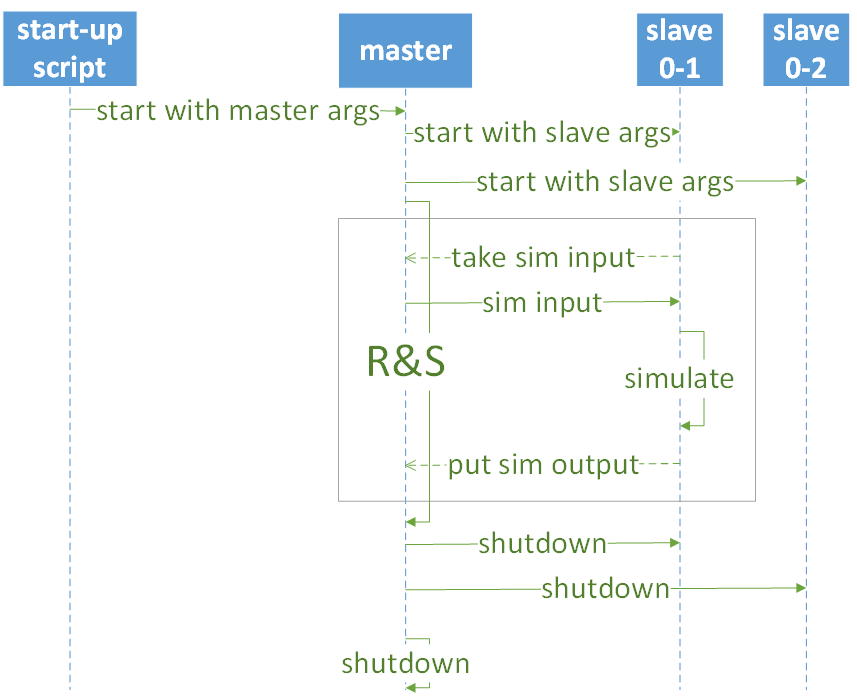
\includegraphics[height=72mm]{overview_seq_single.png}
\end{figure}
\end{frame}

\begin{frame}
\frametitle{Master-Slave Structure}
\framesubtitle{Communication via FIFO Queue}
\begin{figure}[ht]
\centering
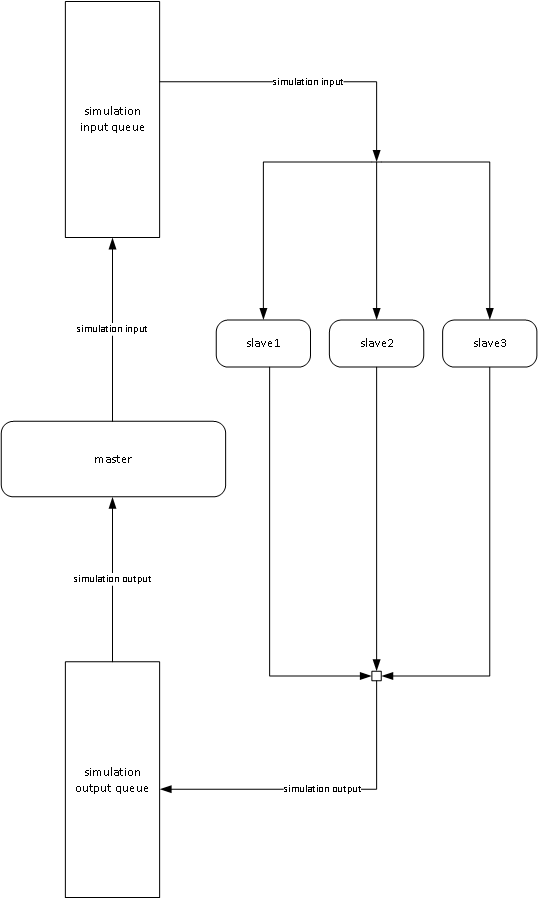
\includegraphics[height=48mm]{master-slave-queue.png}
\end{figure}
\begin{itemize}
\item two producer-consumer problem with existing solution
\item depend on standard component
\end{itemize}
\end{frame}

\begin{frame}
\frametitle{Design for Extension}
\framesubtitle{Partial Class Diagram}
\begin{figure}[ht]
\centering
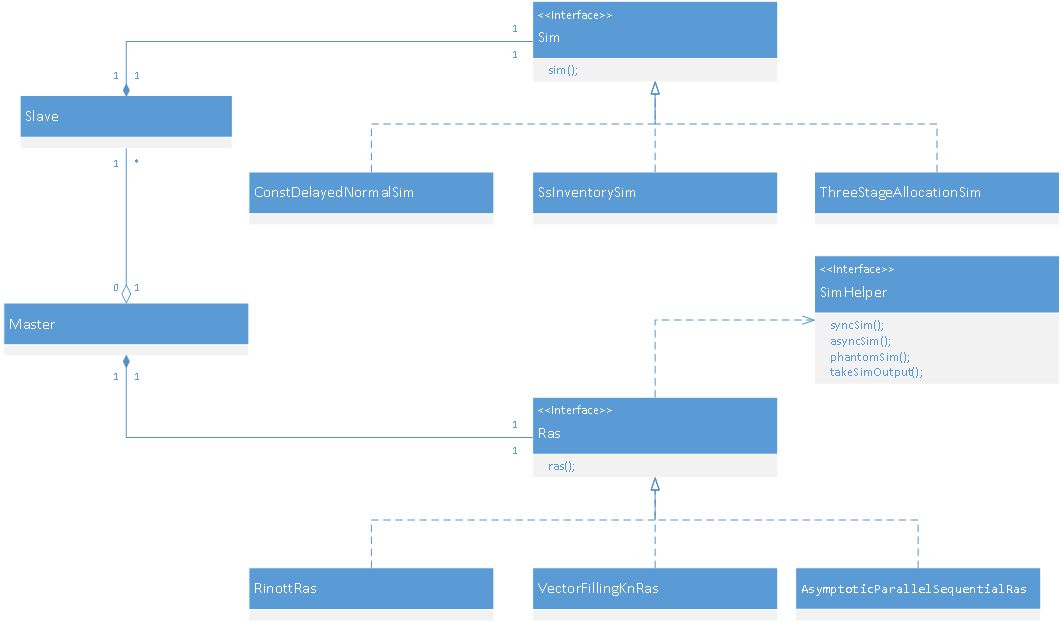
\includegraphics[height=64mm]{ras-sim-class.png}
\end{figure}
\end{frame}

\begin{frame}[fragile]
\frametitle{Design for Extension}
\framesubtitle{Interfaces to Implement}
\begin{itemize}
\item simulation(sim) interface:
\begin{lstlisting}[language=Java]
public double[] sim(double[] alt, double[] args, long[] seed);
\end{lstlisting}
\item ranking-and-selection(ras) interface:
\begin{lstlisting}[language=Java]
public int ras(double[][] alts, double[] args, SimHelper helper);
\end{lstlisting}
\item For example, in $(s, S)$ inventory simulation:
\begin{itemize}
\item $alt$: $[id, s, S]$
\item Sim $args$: $[warmup\_len, running\_len, arrive\_rate...]$
\item $seed$: generated from $master\_seed$
\item $alts$: $[alt1, alt2...]$
\item Ras $args$: $[\alpha, \delta, n_0...]$
\end{itemize}
\end{itemize}
\end{frame}

\begin{frame}[fragile]
\frametitle{Design for Extension}
\framesubtitle{SimHelper interface used for implementing Ras interface}
\begin{lstlisting} [language=Java]
public class SimInput
{
  public int altID;
  public double[] args;
  public long[] seed;
}
\end{lstlisting}
\begin{lstlisting}[language=Java]
public class SimOutput
{
  public int altID;
  public double[] result;
}
\end{lstlisting}
\begin{lstlisting}[language=Java]
public interface SimHelper
{
  public SimOutput[] syncSim(int[] altIDs);
  public int asyncSim(int[] altIDs);
  public int phantomSim(int[] altIDs);
  public SimOupput takeSimOutput();
  public SimOutput[] takeSimOutputs(int n, boolean block);
}
\end{lstlisting}
\end{frame}

\begin{frame}
\frametitle{Illustration of synchronous $sim$ interface}
\framesubtitle{Revisit of the Rinott's Procedure}
\tiny
{
\begin{algorithmic}[1]
\Require $k, \alpha, \delta, n_0$
\State $h \gets$ the Rinott's const with arguments $k, \alpha, n_0$
\State $altIds \gets \{0, 1, 2...k - 1, 0, 1, 2...k - 1...\}$ \Comment{repeat $n_0$ cycles}
\State {\color{blue} SimOutput[] outputs = simHelper.syncSim(altIds);}
\State store {\color{blue} outputs} into $X_{ij}$
\State $altIds2 \gets \emptyset$
\For{$i = 0 \to k - 1$}
  \State $\bar{X_i}(n_0) = \frac{1}{n_0} \sum_{j=0}^{n_0 - 1}X_{ij}$; 
  \State $S_i^2 = \frac{1}{n_0 - 1} \sum_{j=0}^{n_0 - 1}(X_{ij} - \bar{X_i}(n_0))^2$;
  \State $N_i = \max\{n_0, \lceil \frac{h^2S_i^2}{\delta^2} \rceil\}$
  \For{$j = 0 \to (N_0 - n_0) - 1$}
    \State append $i$ into $altIds2$
  \EndFor
\EndFor
\State {\color{blue} SimOutput[] outputs2 = simHelper.syncSim(altIds2);}
\State store {\color{blue} outputs2} into $X_{ij}$
\For{$i = 0 \to k - 1$}
  \State $\bar{X_i}(N_0) = \frac{1}{N_0} \sum_{j=0}^{N_0 - 1}X_{ij}$
\EndFor
\State \Return $\argmax_{i}\bar{X_i}(N_0)$
\end{algorithmic}
}
\end{frame}

\begin{frame}
\frametitle{Illustration of asynchronous $sim$ interface}
\framesubtitle{Revisit of the Vector Filling KN Procedure}
\tiny
{
\begin{algorithmic}[1]
\Require $k, \alpha, \delta, n_0$
\State $h^2 \gets (n_0 -1)[(\frac{2\alpha}{k - 1})^{-2/(n_0-1)} - 1]$
\State $altIds \gets \{0, 1, 2...k - 1, 0, 1, 2...k - 1...\}$ \Comment{repeat $n_0$ cycles}
\State {\color{blue} SimOutput[] outputs = simHelper.syncSim(altIds);}
\State store outputs into $X_{ij}$
\State $survivingCount \gets k$;
\State $r \gets n_0$
\State comparison and elimination
\While{$survivingCount > 1$}
  \State $altIds2 \gets \emptyset$
  \For{$i = 0 \to k - 1$}
    \If{alternative $i$ is still surviving}
      \State append $i$ into $altIds2$
    \EndIf
  \EndFor
  \State {\color{blue}simHelper.asyncSim(altIds);} \Comment{More added simulation input than simulation output taken}
  \State {\color{blue} SimOutput output = simHelper.takeSimOutput();}
  \State store outputs into $X_{ij}$
  \If{$\min{len(X_i)} > r$}
    \State $r \gets r + 1$;
    \State comparison and elimination
  \EndIf
\EndWhile
\State \Return id of the surviving alternative
\end{algorithmic}
}
\end{frame}

\begin{frame}
\frametitle{Illustration of phantom $sim$ interface}
\framesubtitle{Revisit of the Asymptotic Parallel Sequential Procedure}
\tiny
{
\begin{algorithmic}[1]
\Require $k, \alpha, \delta, n_0$
\State $a \gets - \log{[2\alpha / (k - 1)]}$
\State $altIds \gets \{0, 1, 2...k - 1, 0, 1, 2...k - 1...\}$ \Comment{repeat $n_0$ cycles}
\State {\color{blue} SimOutput[] outputs = simHelper.syncSim(altIds);}
\State store outputs into $X_{i\ell}$
\State $survivingCount \gets k$;
\State comparison and elimination
\State $altIds2 \gets \emptyset$
\For{$i = 0 \to k - 1$}
  \If{alternative $i$ is still surviving}
    \State append $i$ into $altIds2$
  \EndIf
\EndFor
\State {\color{blue}simHelper.asyncSim(altIds);}
\State {\color{blue}simHelper.phantomSim(k);}
\While{$survivingCount > 1$}
  \State {\color{blue} SimOutput output = simHelper.takeSimOutput();}
  \State store {\color{blue} outputs} into $X_{i\ell}$
  \If{$simOutput$ is phantom}
    \State $altIds2 \gets \emptyset$
    \For{$i = 0 \to k - 1$}
      \If{alternative $i$ is still surviving}
        \State append $i$ into $altIds2$
      \EndIf
    \EndFor
    \State {\color{blue}simHelper.asyncSim(altIds);}
    \State {\color{blue}simHelper.phantomSim(k);} \Comment{A phantom simulation input won't be taken by slave}
    \State comparison and elimination
  \EndIf
\EndWhile
\State \Return id of the surviving alternative
\end{algorithmic}
}
\end{frame}

\begin{frame}
\frametitle{Logging}
\framesubtitle{To Reproduce Simulation R\&S Procedure}
\begin{itemize}
\item selection result
\item response time
\item input sequence
\begin{itemize}
\item $altId, args, seeds$
\item count of simulation input enqueue and dequeue
\item record of sampling rule
\end{itemize}
\item output sequence
\begin{itemize}
\item $altId, result$, corresponding input info
\item count of simulation output enqueue and dequeue
\item {\color{blue} can be used to reproduce the parallel execution into serial}
\end{itemize}
\end{itemize}
\end{frame}

%\begin{frame}
%\frametitle{Deploy on Cluster}
%\begin{itemize}
%\item Scale-up v.s. Scale-out
%\item agent in charge of communication via network
%\item simulation input management
%\begin{algorithmic}[1]
%\While{\text{true}}
%  \If{$inputQueue.size() < s1$}
%    \State{send request for $(s2 - s1)$ simulation inputs via network}
%    \ForAll{obtained simulation inputs}
%      \State{inputQueue.put(input)}
%    \EndFor
%  \Else
%    \State{sleep for 1 second}
%  \EndIf
%\EndWhile
%\end{algorithmic}
%\item simulation output management (as aggressive as possible)
%\end{itemize}
%\end{frame}

\section{System Evaluation}

\begin{frame}
\frametitle{Comparative Study of Three Parallel Procedures}
\framesubtitle{Nemerical Experiments Setting}
\begin{itemize}
\item {Problem Setting: } \\ 100 normal distributed alternatives, with pre-known mean and variance. One of them has maximum mean 1, others has mean of 0, and all of them has variance of 1.
\vspace{\baselineskip}
\item {Computing Environment: } \\ A local pc with 8 hardware thread, using 4 slaves.
\vspace{\baselineskip}
\item {R\&S Parameters: } \\ $\alpha=0.05, \delta=1, n_0 = 10$.
\end{itemize}
\end{frame}

\begin{frame}
\frametitle{Comparative Study of Three Parallel Procedures}
\framesubtitle{Nemerical Result}
\begin{table}[ht]
\begin{center}
\scalebox{0.6}
{
\begin{tabular}{|c|c|c|c|}
\hline
rep: & Rinott & VFKN & APS \\
\hline
1 & 457533, 457533, 457533, 457533, 3368ms & 23889, 23833, 23832, 3780, 476ms & 1296, 1296, 1296, 1292, 95ms \\
\hline
2 & 467561, 467561, 467561, 467561, 3293ms & 16363, 14981, 14980, 2173, 116ms & 1333, 1333, 1333, 1329, 56ms \\
\hline
3 & 490175, 490175, 490175, 490175, 3356ms & 24061, 17010, 17009, 3050, 138ms & 1265, 1265, 1265, 1262, 47ms \\
\hline
4 & 473949, 473949, 473949, 473949, 3306ms & 16638, 13863, 13862, 2898, 111ms & 1205, 1205, 1205, 1202, 37ms \\
\hline
5 & 446015, 446015, 446015, 446015, 3151ms & 14937, 13771, 13769, 3758, 114ms & 1247, 1247, 1247, 1243, 45ms \\
\hline
\end{tabular}
}
\end{center}
\end{table}
{\tiny In each table cell, the numbers means count of simulation input put, count of simulation input taken, count of simulation output put, count of simulation output taken and total time cost, respectively.}
\begin{itemize}
\item time cost
\item count of enqueue and dequeue operations of two queues
\end{itemize}
\end{frame}

\begin{frame}
\frametitle{Scalability Testing}
\framesubtitle{Numerical Experiments}
\begin{itemize}
\item {Problem Setting: } \\ 21660 alternatives consists the feasible region of a three-stage allocation problem, with 2 best one, and 4 acceptable good one, from IZ viewpoint.
\vspace{\baselineskip}
\item {Computing Environment: } \\ A powerful server with 48 threads.
\vspace{\baselineskip}
\item {R\&S Parameters: } \\ APS procedure with $\alpha=0.05, \delta=1, n_0 = 10$.
\vspace{\baselineskip}
\item {Numerical Results: }
\begin{table}[ht]
\begin{center}
\scalebox{0.85}
{
\begin{tabular}{|c|c|c|c|c|c|c|}
\hline
Num. of Slaves(n): & 1 & 4 & 8 & 16 & 32 & 48 \\
\hline
Sample Size($\times 10^5$) & 2.426 & 2.434 & 2.442 & 2.442 & 2.433 & 2.436\\
\hline
Elapsed Minutes(t): & 370.5 & 129.4 & 94.4 & 68.3 & 41.7 & 34.2 \\
\hline
\end{tabular}
}
\end{center}
\end{table}
\end{itemize}
\end{frame}

\begin{frame}
\frametitle{Scalability Testing}
\framesubtitle{Related Concept and Theory}
\begin{itemize}
\item Speed-up Ratio
$$ S_n = \frac{T_1}{T_n} $$
\item Amdahl's Law
\begin{align*}
S_n & = \frac{1}{(1 - p) + \frac{p}{n}} \\
\lim_{n \to +\infty} S_n & = \lim_{n \to +\infty} \frac{1}{(1 - p) + \frac{p}{n}} = \frac{1}{1 - p}
\end{align*}
\end{itemize}
\end{frame}

\begin{frame}
\frametitle{Scalability Testing}
\framesubtitle{Time cost modeling}
\begin{align*}
t & = a \times (1 - p + \frac{p}{n}) + \epsilon \\
& = (a - ap) + ap \times \frac{1}{n} + \epsilon
\end{align*}
With linear regression, we can get $a - ap = 40.4$ and $ap = 332.9$ with $R^2 \geqslant 0.994$, so $p$ is 0.892, which means roughly $89.2\%$ of simulation work is paralleled.
\end{frame}

\section{Implementation Acceleration}

\begin{frame}
\frametitle{Revist of the APS Procedure}
\framesubtitle{Comparing and Elimination}
What will happen with a new sample value / a new updated alternative?
$$ \bar{X_{i}}(N_{ir}) - \bar{X_{j}}(N_{jr}) < \min\{0, -\frac{a}{\delta}[\frac{S_i^2(N_{ir})}{N_{ir}} + \frac{S_j^2(N_{jr})}{N_{jr}}] + \frac{\delta}{2}\} $$
Checking elimination literately with linear complexity?
\begin{itemize}
\item A bottle-neck when simulation is fast enough to make output queue always non-empty.
\item Limiting the scalability of the whole system, since it's about the serial part.
\end{itemize}
\end{frame}

%\begin{frame}
%\frametitle{Async Rinott}
%\tiny
%{
%\begin{algorithmic}[1]
%\Require $k, \alpha, \delta, n_0$
%\State $h \gets$ the Rinott's const with arguments $k, \alpha, n_0$
%\State $altIds \gets \{0, 1, 2...k - 1, 0, 1, 2...k - 1...\}$ \Comment{repeat $n_0$ cycles}
%\State {\color{blue}simHelper.asyncSim(altIds);}
%\State $sCount \gets k \times n_0$ \Comment{sCount: sampling count}
%\State initialize $count[k], sum[k], sos[k]$ \Comment{sos: sum of square}
%\While {$sCount > 0$}
%  \State {\color{blue} SimOutput output = simHelper.takeSimOutput();}
%  \State update corresponding $count[i], sum[i], sumOfSquare[i]$
%  \State $sCount \gets sCount - 1$
%  \If{$count[i] = n_0$}
%	\State $mean \gets sum[i] / count[i]$
%	\State $S2 \gets (sos[i] - count[i] \times mean^2) / (count[i] - 1)$
%	\State $N \gets \max\{n_0, \lceil \frac{h^2S2}{\delta^2} \rceil\}$
%	\If{$N > n_0$}
%	  \State $altIds2 \gets \emptyset$
%      \For{$j = 0 \to (N - n_0) - 1$}
%        \State append $i$ into $altIds2$
%      \EndFor
%      \State {\color{blue}simHelper.asyncSim(altIds2);}
%	  \State $sCount \gets sCount + (N - n_0)$
%	\EndIf
%  \EndIf
%\EndWhile
%\State \Return $\argmax_{i} sum[i] / count[i]$
%\end{algorithmic}
%}
%\end{frame}
%
%\begin{frame}
%\frametitle{Comment of Async Rinott Procedure}
%\begin{itemize}
%\item Numerical experiment end with a non-positive result, not too much difference compared with the classic Rinott's procedure.
%\vspace{\baselineskip}
%\item Omitting a barrier saves the time cost of one simulation at most, since a barrier will wait for the slowest simulation. But during Rinott's procedure we need many simulations in total, even for a very small $k$.
%\vspace{\baselineskip}
%\item It provides a trial combining staged procedure and sequential procedure, and reminds us that some barriers in existing procedures are not necessary.
%\end{itemize}
%\end{frame}

\begin{frame}
\frametitle{Heaped APS}
\framesubtitle{Introduction of Heap}
\begin{figure}[ht]
\centering
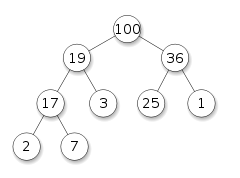
\includegraphics[height=32mm]{heap.png}
\end{figure}
\begin{itemize}
\item insert node with certain key value: $O(\log n)$
\item find node with min(max) key value: $O(1)$
\item update key value of certain node after the node is located: $O(\log n)$
\item remove node with min(max) key value: $O(\log n)$
\item find node with {\bf arbitrary} key value: $O(n)$
\vspace{\baselineskip}
\item {\color{blue} in our scenario, find node representing any alternative: $O(1)$}
\end{itemize}
\end{frame}

%\begin{frame}
%\frametitle{Heaped APS}
%\framesubtitle{$O(1)$ Query for Arbitrary Key Value in Heap}
%\begin{figure}[ht]
%\centering
%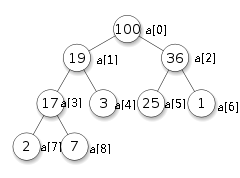
\includegraphics[height=32mm]{heap2.png}
%\end{figure}
%\begin{itemize}
%\item The two children nodes of node $a[i]$ can be represented as $a[2 \times i + 1]$ and $a[2 \times i + 2]$, if exists.
%\item Track internal location of each node!
%\end{itemize}
%\end{frame}

\begin{frame}
\frametitle{Heaped APS}
\framesubtitle{Heaped Comparison with A New Sample}
$$ \bar{X_{i}}(N_{ir}) - \bar{X_{j}}(N_{jr}) < \min\{0, -\frac{a}{\delta}[\frac{S_i^2(N_{ir})}{N_{ir}} + \frac{S_j^2(N_{jr})}{N_{jr}}] + \frac{\delta}{2}\} $$
To see whether $ -\frac{a}{\delta}[\frac{S_i^2(N_{ir})}{N_{ir}} + \frac{S_j^2(N_{jr})}{N_{jr}}] + \frac{\delta}{2} > 0$, check alt with largest $\frac{S^2(N_r)}{N_r}$.
\begin{align*}
& \bar{X_{i}}(N_{ir}) - \bar{X_{j}}(N_{jr}) < -\frac{a}{\delta}[\frac{S_i^2(N_{ir})}{N_{ir}} + \frac{S_j^2(N_{jr})}{N_{jr}}] + \frac{\delta}{2} \\
\Longrightarrow & \bar{X_{i}}(N_{ir}) + \frac{a}{\delta}\frac{S_i^2(N_{ir})}{N_{ir}} < \bar{X_{j}}(N_{jr}) - \frac{a}{\delta}\frac{S_j^2(N_{jr})}{N_{jr}} + \frac{\delta}{2}
\end{align*}
\begin{itemize}
\item Check alt with smallest $\bar{X}(N_r) + \frac{a}{\delta}\frac{S^2(N_r)}{N_r}$, to see whether the updated alternative will eliminate others, with iteration.
\item Check alt with largest $\bar{X}(N_r) - \frac{a}{\delta}\frac{S^2(N_r)}{N_r}$, to see whether the updated alternative is eliminated by others, without iteration.
\end{itemize}
\end{frame}

\begin{frame}
\frametitle{Heaped APS}
\framesubtitle{Heaped Comparing Algorithm}
\begin{algorithmic}[1]
\tiny
{
\Require $simOutput$, including corresponding $altId$ and $value$ of output
\State $alt = alts0[altId]$ \Comment{$alts0$ is an array of alternative objects, $O(1)$}
\If{$alt.isSurviving() = false$} 
  \State \Return
\EndIf
\State $alts.addSample(value)$ \Comment{update $N, \bar{X}(N), S^2(N)$ e.g. $O(1)$}
\State adjust heap $alts1$, $alts2$, $alts3$, {\color{blue} where $alts1$ is a max-heap with key $S^2(N)/N$, $alts2$ is a min-heap with key $\bar{X}(N) + \frac{a}{\delta}\frac{S^2(N)}{N}$, $alts3$ is a max-heap with key $\bar{X} - \frac{a}{\delta}\frac{S^2(N)}{N}$} \Comment{heap adjustment involved, $O(\log k)$}
\State $alt1 = alts1.peek()$
\While {$alt.key1() + alt1.key1() < \frac{\delta^2}{2a}$}
  \If{alt.mean() < alt1.mean()}
    \State eliminate $alt$ and \Return \Comment{heap adjustment involved, $O(\log k)$}
  \Else
    \State eliminate $alt1$ and $alt1 = alts1.peek()$ \Comment{heap adjustment involved, $O(\log k)$}
  \EndIf
\EndWhile
\State $alt2 = alts2.peek()$
\While{$alt2.key2() < alt.key3()$}
  \State eliminate $alt2$ and $alt2 = alts2.peek()$ \Comment{heap adjustment involved, $O(\log k)$}
\EndWhile
\State $alt3 = alts3.peek()$
\If{$alt.key2() < alt3.key3()$}
  \State eliminate $alt$ and \Return \Comment{heap adjustment involved, $O(\log k)$}
\EndIf
}
\end{algorithmic}
\end{frame}

\begin{frame}
\frametitle{Heaped Comparing Algorithm}
\framesubtitle{Substantial Accelaration of Serial Part}
\begin{itemize}
\item {Problem Setting: } \\ Variant number of normal distributed alternatives, with pre-known mean and variance. One of them has maximum mean 1, others has mean of 0, and all of them has variance of 1.
\item {Computing Environment: } \\ A local pc with 8 hardware thread, using 4 slaves. Simulation output queue is always non-empty.
\item {R\&S Parameters: } \\ APS and HAPS procedure with $\alpha=0.05, \delta=1, n_0 = 10$.
\item {Numerical Results: }
\begin{table}[ht]
\begin{center}
\scalebox{0.85}
{
\begin{tabular}{|c|c|c|c|c|c|c|}
\hline
Num. of Alternatives(k): & 100 & 1000 & 10000 & 100000 \\
\hline
Linear Comparison (ms): & 56 & 199.6 & 5606.4 & 884992.6 \\
\hline
Heaped Comparison (ms): & 54.8 & 163.6 & 906 & 10338.6 \\
\hline
\end{tabular}
}
\end{center}
\end{table}
\end{itemize}
\end{frame}

\section{Conclusion}

\begin{frame}
\frametitle{Conclusion}
\begin{itemize}
\item Our framework has achieved good scalability with most workload being carried out in parallel.
\vspace{\baselineskip}
\item Our framework has exposed proper programming interfaces, making it easy to develop new procedures on top of it.
\vspace{\baselineskip}
\item Our comparison algorithm within APS procedure has achieved better time complexity than naive linear, which further improve the system performance by decreasing workload that has to be in serial.
\end{itemize}
\end{frame}

%\begin{frame}
%\frametitle{Related Work}
%\begin{itemize}
%\item simulation R\&S procedure: traditionally focus on statistical validity
%\vspace{\baselineskip}
%\item parallel and distributed simulation(PADS): accelerating single extremely long simulation experiment
%\vspace{\baselineskip}
%\item optimization via simulation(OvS): sacrificing statistical validity for dealing with larger problem size in serial computing environment
%\end{itemize}
%\end{frame}
%
%\begin{frame}
%\frametitle{Future Work}
%\begin{itemize}
%\item system viewpoint
%\begin{itemize}
%\item scale out: centralized v.s. decentralized (see \cite{potwsc05ras})
%\item task scheduling: task-pool v.s. explicit scheduler
%\end{itemize}
%\item implementation viewpoint
%\begin{itemize}
%\item algorithm complexity: more rigorous analysis of heaped comparing
%\item sample processing: single v.s. batched
%\end{itemize}
%\item application viewpoint
%\begin{itemize}
%\item we lack a comparative study of parallel procedures (see \cite{ms05ras})
%\item providing service as cloud computing and become benchmark
%\end{itemize}
%\item others
%\begin{itemize}
%\item we lack a thread-safe discrete-event simulation library (see \cite{ssj})
%\end{itemize}
%\end{itemize}
%\tiny
%{
%\begin{thebibliography}{10}
%\bibitem{potwsc05ras} Chen, E. J. Using parallel and distributed computing to increase the capability of selection procedures. In Proceedings of the 2005 Winter Simulation Conference, pp. 723–731.
%\bibitem{ms05ras} Jurgen Branke, Stephen E. Chick, Christian Schmidt. Selecting a Selection Procedure. Management Science, 2005.
%\bibitem{ssj} Lecuyer Pierre, Simard Richard, Chen E. Jack, Kelton W. David. An Object-Oriented Random-Number Package with Many Long Streams and Substreams. Operations Research, 2002.
%\end{thebibliography}
%}
%\end{frame}

\begin{frame}
\begin{center}
\Huge \bf \color{blue} THANK YOU!
\end{center}
\end{frame}

\end{document}
